\subsection*{Aufgabe 15}
Wahrscheinlichkeiten f�r ein Ereignis lassen sich approximieren, indem man das
entsprechende Zufallsexperiment h�ufig durchf�hrt und die relative H�ufigkeit betrachtet, mit
der das Ereignis eintritt. Nat�rlich f�hrt man das Experiment nicht wirklich durch, sondern
l�sst es den Rechner simulieren. Wir betrachten zun�chst die Lotto-Ziehung, bei der 6 aus 49
Zahlen ohne Zur�cklegen ausgew�hlt werden.
\begin{enumerate} [leftmargin=0.5cm, label=\alph*)]
\item Mit welcher Wahrscheinlichkeit ist die kleinste der 6 ausgew�hlten Zahlen gleich 17?
(Hinweis: �berlegen Sie, wie viele Ziehungen es gibt, bei denen die 17 und zus�tzlich 5
Zahlen zwischen 18 und 49 gezogen werden.)
\item Das Ergebnis aus a) wollen wir nun durch Simulation �berpr�fen. Der entscheidende R-Befehl
ist $sample(N,n)$: \newline \newline
$sample(N,n)$ erzeugt einen Vektor, der eine zuf�llige Ziehung ohne Zur�cklegen von n
Elementen aus den ganzen Zahlen von 1 bis N simuliert. \newline \newline
$sample(N, n, replace = T)$ zieht mit Zur�cklegen, \newline \newline
$sample(N,N)$ erzeugt eine zuf�llige Permutation der ganzen Zahlen von 1 bis N. \newline \newline
Betrachten Sie folgenden R-Code:
\begin{center}
\begin{figure}[!htbp]
\fbox{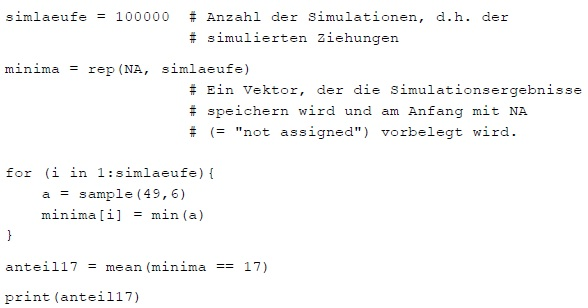
\includegraphics[width=0.9\textwidth,page=1]{chapters_AB/Grafiken_AB/AB_3_15.jpg}}
\end{figure}
\end{center}
\end{enumerate}
Versuchen Sie zu verstehen, was in jedem Schritt passiert. Lassen Sie den Code mehrmals
ausf�hren und beobachten Sie, welche Nachkommastellen des Ergebnisses stabil bleiben.
Erh�hen oder verkleinern Sie den Wert von $simlaeufe$, und beobachten Sie die
Ergebnisse. Vergleichen Sie mit Ihrem Ergebnis aus a).
